\CVioBeginChapter{1}{I. Project Introduction}
\section{Overview}
\subsection{Project Information}
This subsection records the institutional and academic context of the project. Project Title: Lightweight Deep Learning for Robust Shrimp Disease Detection on Mobile Devices under Diverse Environmental Conditions. Project Code: AIP491\_01. Group Name: CVio. Academic Program: Bachelor of Artificial Intelligence. Department: Department of Artificial Intelligence. Institution: FPT University - Campus Can Tho. Supervisor: Nguyen Dinh Vinh. Project Team: Tran Huu Nhan, Le Thi Huynh Nhu, and Nguyen Van Phong.\par
\begingroup
\CVioTableSetup
\begin{longtable}{|>{\centering\arraybackslash}p{2.79cm}|>{\centering\arraybackslash}p{7.96cm}|}
\caption{Project information}\\
\hline
\rowcolor{cvioPeach}\textbf{Item} & \textbf{Information} \\ \hline
\endfirsthead
\caption[]{Project information (continued)}\\
\hline
\rowcolor{cvioPeach}\textbf{Item} & \textbf{Information} \\ \hline
\endhead
\hline
\multicolumn{2}{r}{\footnotesize Continued on next page}\\
\endfoot
\hline
\endlastfoot
\rev{English project name} & \rev{Lightweight Deep Learning for Robust Shrimp Disease Detection on Mobile Devices under Diverse Environmental Conditions} \\ \hline
\rev{Vietnamese project name} & \rev{Phát hiện bệnh tôm bằng mô hình học sâu nhẹ trên thiết bị di động trong nhiều điều kiện môi trường khác nhau} \\ \hline
\rev{Project code} & \rev{AIP491\_01} \\ \hline
\rev{Group name} & \rev{CVio} \\ \hline
\rev{Academic program} & \rev{Bachelor of Artificial Intelligence} \\ \hline
\rev{Department} & \rev{Department of Artificial Intelligence} \\ \hline
\rev{Institution} & \rev{FPT University - Campus Can Tho} \\ \hline
\rev{Project type} & \rev{AI-based four-class image classification, BG/WSSV instance segmentation, robustness and explainability evaluation, deployment-oriented lightweight-model research, native Android application development, and Firebase-backed data integration} \\ \hline
\rev{Software type} & \rev{Native Android mobile application with integrated artificial-intelligence and data-management functions} \\ \hline
\rev{Target platform} & \rev{Android application using a conditional two-model TensorFlow Lite/LiteRT cascade on the common CPU execution path, with Firebase data services} \\ \hline
\rev{Main AI tasks} & \rev{Four-class shrimp disease image classification and BG/WSSV disease-region instance segmentation, with Healthy retained as an empty-label segmentation negative} \\ \hline
\rev{Main technologies} & \rev{Python, PyTorch, TorchVision, Ultralytics, OpenCV, Jupyter/Kaggle Notebook, TensorFlow Lite/LiteRT, Kotlin, Android Studio, Firebase, Git, and GitHub} \\ \hline
\end{longtable}
\endgroup
\rev{
Table 1.1 establishes that the project is primarily an AI research project with a mobile application as its deployment layer. The final application packages the classifier and instance-segmentation model as one conditional Android inference cascade; the project outcome therefore combines classification, localization, robustness, explainability, model-efficiency, and operational deployment evidence rather than treating the mobile prototype as the sole research contribution.
}
\begingroup
\CVioTableSetup
\begin{longtable}{|>{\centering\arraybackslash}p{2.92cm}|>{\centering\arraybackslash}p{3.47cm}|>{\centering\arraybackslash}p{1.90cm}|>{\centering\arraybackslash}p{2.45cm}|}
\caption{Supervisor information}\\
\hline
\rowcolor{cvioPeach}\textbf{Full Name} & \textbf{Email} & \textbf{Mobile} & \textbf{Title} \\ \hline
\endfirsthead
\caption[]{Supervisor information (continued)}\\
\hline
\rowcolor{cvioPeach}\textbf{Full Name} & \textbf{Email} & \textbf{Mobile} & \textbf{Title} \\ \hline
\endhead
\hline
\multicolumn{4}{r}{\footnotesize Continued on next page}\\
\endfoot
\hline
\endlastfoot
Nguyen Dinh Vinh & vinhnd29@fe.edu.vn & 0975894685 & Lecturer / Supervisor \\ \hline
\end{longtable}
\endgroup
\begingroup
\CVioTableSetup
\begin{longtable}{|>{\centering\arraybackslash}p{2.86cm}|>{\centering\arraybackslash}p{3.40cm}|>{\centering\arraybackslash}p{1.90cm}|>{\centering\arraybackslash}p{2.58cm}|}
\caption{Team member information}\\
\hline
\rowcolor{cvioPeach}\textbf{Full Name} & \textbf{Email} & \textbf{Mobile} & \textbf{Role} \\ \hline
\endfirsthead
\caption[]{Team member information (continued)}\\
\hline
\rowcolor{cvioPeach}\textbf{Full Name} & \textbf{Email} & \textbf{Mobile} & \textbf{Role} \\ \hline
\endhead
\hline
\multicolumn{4}{r}{\footnotesize Continued on next page}\\
\endfoot
\hline
\endlastfoot
Tran Huu Nhan (CE181655) & nhanthce181655@fpt.edu.vn & 0867950216 & Project Leader \\ \hline
Le Thi Huynh Nhu (CA182007) & nhulthca182007@fpt.edu.vn & 0376387478 & Member \\ \hline
Nguyen Van Phong (CE192081) & phongnv.ce192081@gmail.com & 0342324690 & Member \\ \hline
\end{longtable}
\endgroup
Tables 1.2 and 1.3 preserve the official project-contact information. The supervisor provides research direction and milestone assessment, while the project leader coordinates schedule, technical integration, reproducibility, and final document delivery.\par
\subsection{\rev{Project Overview}}
\rev{
This project investigates lightweight computer-vision methods for preliminary shrimp disease screening from images through two connected AI tracks. The classification track predicts Healthy, Black Gill disease (BG), White Spot Syndrome Virus (WSSV), or the WSSV\_BG co-infection category. The instance-segmentation track localizes visible BG and WSSV disease regions. Healthy remains an image-level classification category but is not a positive segmentation class; Healthy images carry no BG/WSSV polygons and are retained in segmentation training, validation, and testing as empty-label negatives.
}
\rev{
The final application implements these tracks as a conditional two-model Android cascade. The FP32 classifier executes first for every accepted image. A Healthy result above the application threshold, or any below-threshold output, terminates the workflow after classification. An above-threshold BG, WSSV, or WSSV\_BG output dispatches the FP16 instance-segmentation model, which produces only BG and WSSV mask instances. This dispatch rule controls application execution and must not be interpreted as verified disease ground truth.
}
The project began with an approved scope centered on four-class classification, robustness evaluation under noisy conditions, lightweight mobile-edge deployment, and optional explainable-AI analysis. Instance segmentation was not part of the initially approved scope. It was added formally after the first review in Session 3 because classification alone was considered insufficient for the expected research depth. Later sessions introduced grouped-specimen splitting, attention-based segmentation refinement, Fourier-domain analysis, external dataset evaluation, and full Android/Firebase integration.\par
\rev{
For segmentation validity, specimen grouping is enforced where specimen identity can be recovered from compatible filenames. Additional unmatched-name images do not expose compatible specimen identifiers and therefore cannot be claimed as specimen-grouped. The expanded segmentation inventory is consequently interpreted with an explicit grouping boundary rather than as fully specimen-leakage-free. Later controlled extensions also evaluate attention placement and Fourier-domain behavior.
}
\rev{
Operational deployment evidence includes a retained 21-image real-world acquisition set collected across the three members’ phone cameras and runtime observations from three Android devices using the common application/model bundle. The images cover variation in illumination, viewpoint, orientation, background clutter, and blur/softness. One unusably dark image was excluded. Because these photographs have no veterinary or laboratory ground truth, they support an operational case study rather than field disease-accuracy validation.
}
Figure 1.1 summarizes the chronological expansion of the project. The leftmost stage represents the initially approved classification scope; the middle stages show the review-driven addition of instance segmentation and later methodological refinements; the final stage presents the integrated research and deployment scope.\par
\begin{figure}[tbp]
\centering
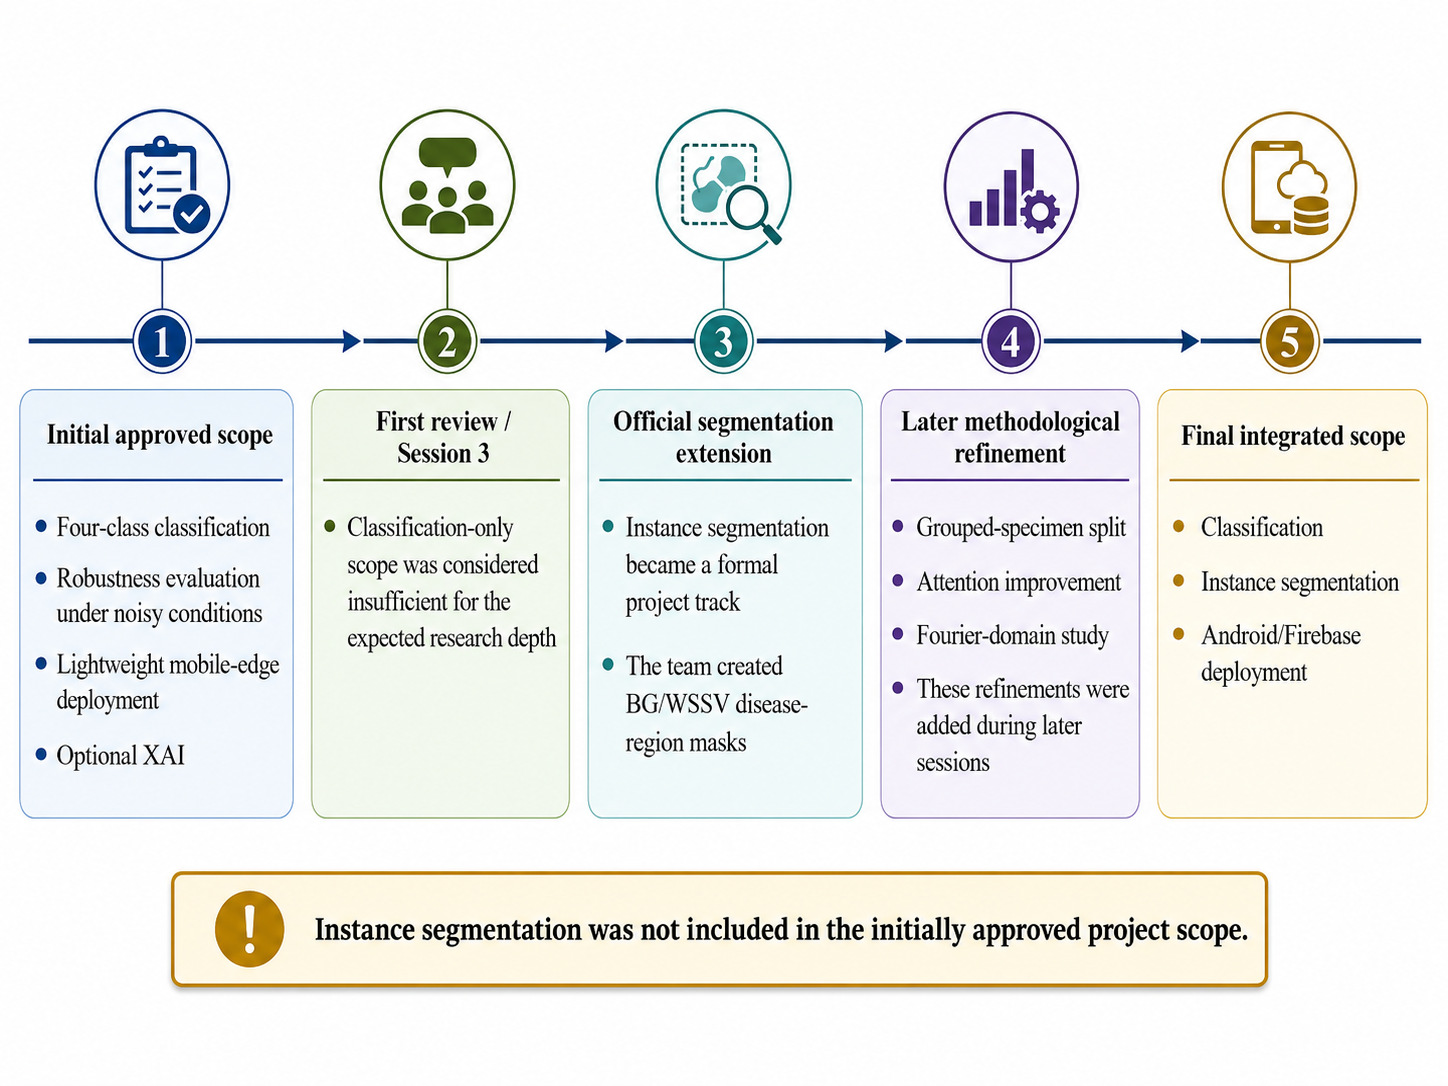
\includegraphics[width=0.94\textwidth,height=0.62\textheight,keepaspectratio]{assets/chapters_1_2/figure_1_1_scope_evolution.png}
\caption{Evolution of the project scope.}
\end{figure}
The figure is important for scope interpretation because it prevents the later segmentation work from being misrepresented as part of the original proposal. It also shows that grouped splitting, attention improvement, and Fourier-domain analysis were controlled scope extensions introduced after the segmentation track had become official.\par
\rev{
Figure 1.1 should be read as a scope-evolution diagram rather than a post-defense chronology. Formal submission and Council-revision milestones are documented in Chapter II. The figure’s purpose here is to distinguish the initially approved classification scope from the later formal segmentation track and its controlled methodological extensions.
}
Figure 1.2 organizes the technologies by their actual function in the project. AI development tools are separated from experimentation infrastructure, mobile deployment technologies, and collaboration services so that the role of each technology is explicit.\par
\begin{figure}[tbp]
\centering
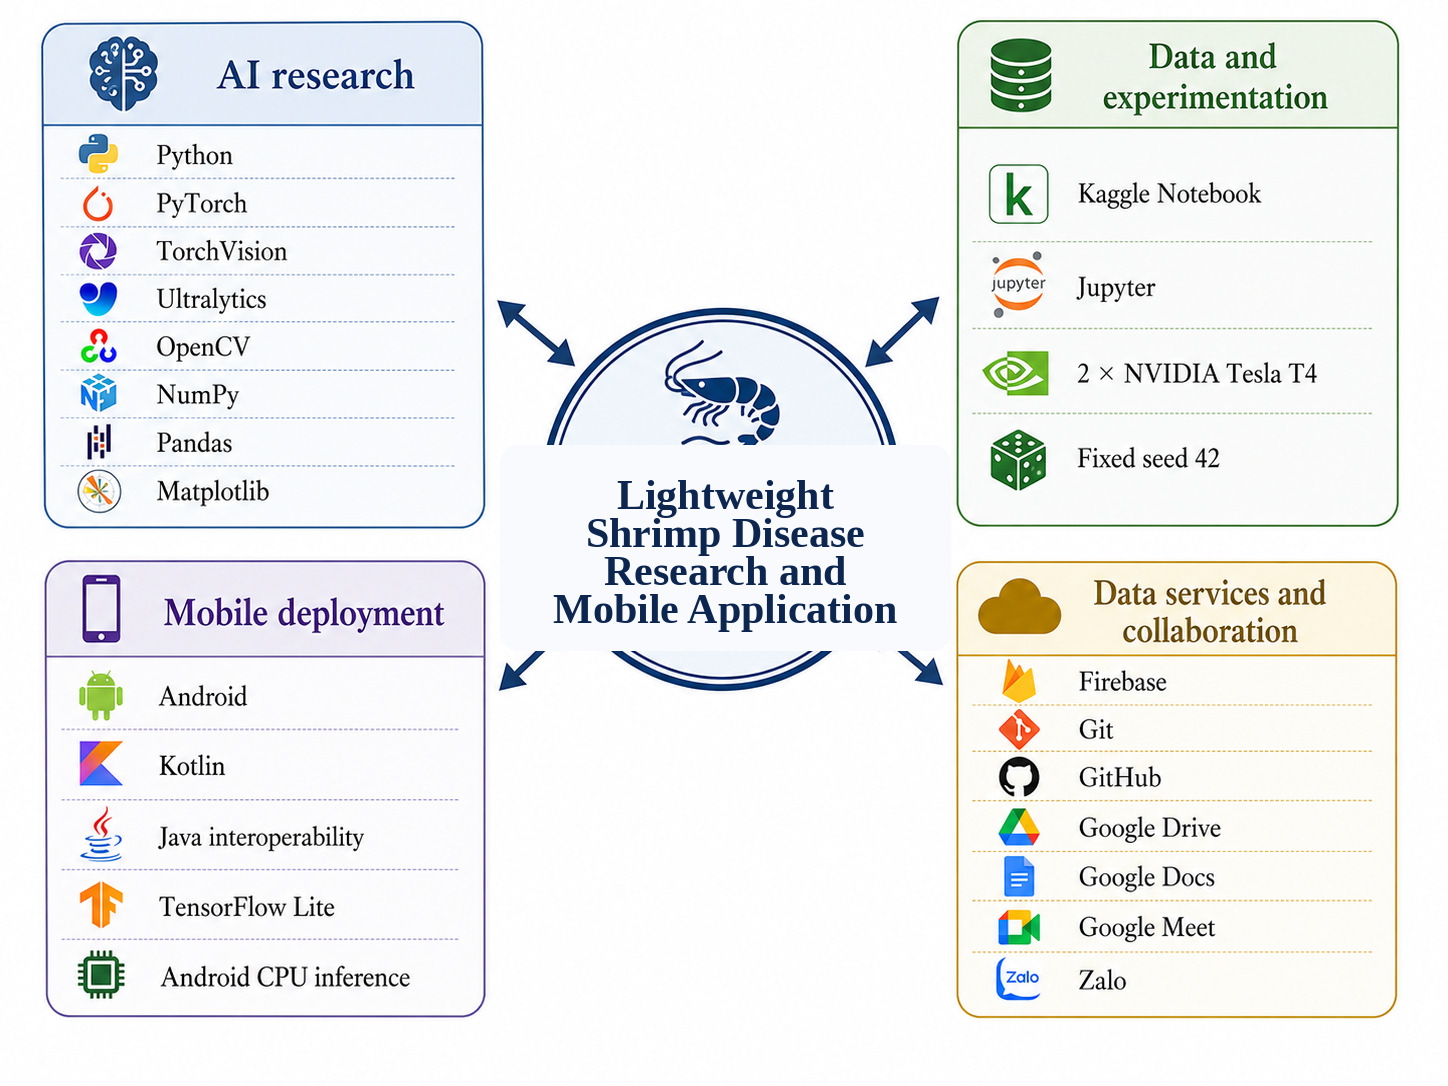
\includegraphics[width=0.94\textwidth,height=0.62\textheight,keepaspectratio]{assets/chapters_1_2/figure_1_2_technology_stack.png}
\caption{Project technology stack.}
\end{figure}
\rev{
The technology stack supports a traceable path from dataset preparation and model experimentation to Android inference and research-asset management. Kaggle/Jupyter and the accepted dual NVIDIA Tesla T4 training environment support reproducible experimentation; PyTorch and Ultralytics support model development; TensorFlow Lite/LiteRT and Android provide the deployment path; and GitHub, Google Drive, Google Docs, Google Meet, Firebase, and Zalo support controlled collaboration and application services. Training hardware, notebook/GPU timing, and Android application runtime are treated as separate provenance categories and are not numerically conflated.
}
\section{\rev{Project Background}}
\rev{
Shrimp aquaculture is economically important, while infectious disease can disrupt production and farm operations. White spot disease is formally associated with infection by white spot syndrome virus (WSSV), for which aquatic-animal-health standards provide dedicated diagnostic methods. Image-based computer vision can therefore support preliminary visual screening, but it is not equivalent to veterinary or laboratory confirmation and must be interpreted within that boundary. can reduce irrelevant cues for classification, but it is not automatically beneficial for segmentation because contextual boundaries and local disease regions may be altered or removed.
}
\rev{
The project also addresses evaluation validity. Repeated views of one physical shrimp can produce optimistic localization estimates if random image-level splitting places related views in both training and testing partitions. Specimen grouping is therefore used where specimen identity is recoverable, while unmatched-name additions are explicitly separated because their filenames do not support specimen-level grouping. This distinction prevents the expanded inventory from being overstated as fully leakage-free.
}
\rev{
Mobile deployment provides an operational path for local preliminary screening. The final Android implementation uses a conditional classifier-to-segmentation cascade rather than executing both models for every image. Consequently, application runtime depends on which branch is executed; operational phone measurements are not automatically equivalent to isolated neural-network latency or to a controlled hardware benchmark.
}
\section{\rev{Project Objective}}
\rev{
The main objective is to design, evaluate, document, and deploy a lightweight deep-learning system for shrimp disease screening that combines class-balanced classification, disease-region localization, robustness analysis, reproducibility, and mobile-oriented operational feasibility. The measurable objectives are as follows:
}
\begin{enumerate}
\item Organize and preprocess public shrimp disease image datasets using fixed and traceable data protocols.
\item \rev{Benchmark representative TIMM and official Ultralytics YOLO classification models and justify the selected deployment-oriented classifier under a preferred budget of approximately 15 million parameters or fewer; larger models may be retained as higher-capacity diagnostic controls rather than eligible final mobile candidates.}
\item \rev{Improve the selected YOLO26m-cls backbone using ASL-LDAM and SimAM-DCFR, with Macro-F1 as the primary classification metric.}
\item Evaluate the selected classifier on the clean test set, controlled synthetic corruption conditions, qualitative explainability visualizations, the separately trained EXT-3-Original regime, and the SDI-4 + EXT-3-Original partition-wise integrated retraining regime.
\item Create BG and WSSV disease-region masks for instance segmentation while retaining Healthy images as empty-label negative samples in training, validation, and testing.
\item \rev{Apply specimen-grouped splitting where specimen identity is recoverable, quantify leakage-prone image-level alternatives, and document the grouping boundary for unmatched-name additions whose filenames do not expose compatible specimen identities.}
\item Evaluate attention-based and Fourier-domain segmentation improvements against controlled baselines.
\item \rev{Convert and integrate the final classification and conditional instance-segmentation artifacts into one native Android inference cascade using TensorFlow Lite/LiteRT, and assess branch-aware operational runtime on real Android devices.}
\item Implement user and administrator workflows with authentication, camera/gallery input, prediction display, mask display, history, export/delete operations, and Firebase integration.
\item Maintain reproducible datasets, configurations, checkpoints, metrics, figures, and thesis evidence through controlled research-asset management.
\end{enumerate}
\section{\rev{Problem Statement}}
\rev{
The project addresses the problem of developing a lightweight shrimp disease image-analysis system that balances class-balanced classification, disease-region instance localization, corruption robustness, repeated-specimen leakage control, model compactness, reproducibility, and mobile deployment feasibility. Strong performance on one clean split is insufficient if the model fails under acquisition disturbances, relies on spurious background cues, produces excessive disease predictions on Healthy negatives, or benefits from leakage between related specimen views. Conversely, model capacity alone cannot define lightweight suitability for an Android deployment target.
}
\rev{
The research problem is therefore multi-objective rather than a single-rank accuracy problem. Candidate selection must consider predictive quality together with parameter efficiency, negative-image behavior, protocol validity, and application-level execution constraints. The final mobile system adds a further systems consideration: classification always executes, whereas instance segmentation is conditional, so observed runtime depends on branch composition. Real-world three-camera photographs and three-device Android observations strengthen operational evidence, but the absence of veterinary/laboratory ground truth means they do not establish prospective field disease accuracy.
}
\rev{
Accordingly, the application is presented as preliminary image-based screening and research demonstration rather than clinical diagnosis. All conclusions remain bounded by the documented datasets, annotation protocol, split construction, corruption tests, and deployment measurements.
}
\section{\rev{Significance of the Project}}
\rev{
Scientifically, the project integrates four-class image classification and BG/WSSV disease-region instance segmentation within one controlled shrimp-disease study. It combines imbalance-aware classification, leakage-aware segmentation, corruption testing, qualitative explainability, attention-placement analysis, Fourier-domain diagnostics, and reproducible artifact management. This structure enables model-selection decisions to be supported by multiple evidence dimensions rather than by one aggregate metric.
}
\rev{
Practically, the project demonstrates a complete Android conditional cascade in which the classifier executes first and the segmentation model is invoked only for above-threshold disease outputs. The same application/model bundle was exercised across three Android devices, and the retained real-world image set was collected from three phone cameras under varied acquisition conditions. These observations demonstrate operational feasibility, but they do not prove farm-ready performance, clinical validity, universal device behavior, or iOS support.
}
\section{\rev{Project Scope and Limitations}}
\rev{
This section defines the work completed within the project and the boundaries that constrain interpretation. The initial proposal focused on four-class classification, robustness under noisy conditions, lightweight mobile-edge deployment, and optional explainability. Instance segmentation was later formalized as a required research track, followed by leakage-aware splitting, attention/Fourier in- vestigations, additional-source classification experiments, and integrated Android/Firebase deployment.
}
\subsection{\rev{Project Scope}}
\rev{
The completed project contains two connected AI research tracks and one deployment layer. The classification track predicts Healthy, BG, WSSV, and WSSV\_BG, with Macro-F1 used as the principal model-ranking metric. The instance-segmentation track predicts BG and WSSV disease-region masks. Healthy is not a segmentation mask class; Healthy images are retained as empty-label negatives.
}
\rev{
Classification external-evidence protocols distinguish three regimes. SDI-4 is the primary four-class classification regime. EXT-3-Original is a separately trained three-class source mapped to Healthy, BG, and WSSV. The SDI-4 + EXT-3-Original regime is a four-class integrated retraining experiment in which each source is split independently before train partitions are merged with train partitions, validation with validation, and test with test; WSSV\_BG is supplied only by SDI-4. The integrated regime is therefore retraining rather than zero-shot external inference.
}
\rev{
The deployment scope integrates the final classifier and the conditional instance-segmentation model into one native Android application using the common TensorFlow Lite/LiteRT model bundle and Firebase-backed user/administrator workflows. The deployment study includes application-recorded branch-aware runtime observations on three Android devices and a 21-image three-camera operational acquisition set. Detailed experimental protocols remain in Chapter IV, and numerical outcomes remain in Chapter VI.
}
\begingroup
\CVioTableSetup
\begin{longtable}{|>{\centering\arraybackslash}p{2.11cm}|>{\centering\arraybackslash}p{4.08cm}|>{\centering\arraybackslash}p{4.56cm}|}
\caption{Final project scope and explicit limitations}\\
\hline
\rowcolor{cvioPeach}\textbf{Scope component} & \textbf{Included work} & \textbf{Boundary / limitation} \\ \hline
\endfirsthead
\caption[]{Final project scope and explicit limitations (continued)}\\
\hline
\rowcolor{cvioPeach}\textbf{Scope component} & \textbf{Included work} & \textbf{Boundary / limitation} \\ \hline
\endhead
\hline
\multicolumn{3}{r}{\footnotesize Continued on next page}\\
\endfoot
\hline
\endlastfoot
\rev{Classification} & \rev{Predict Healthy, BG, WSSV, and WSSV BG from shrimp images; \_ Macro-F1 is the principal ranking metric.} & \rev{Evidence is limited to the documented datasets, source regimes, splits, and accepted checkpoints; it does not establish universal field generalization.} \\ \hline
\rev{Instance segmentation} & \rev{Predict BG and WSSV disease-region masks; retain Healthy images as empty-label negatives.} & \rev{Masks were produced by a single annotator without independent expert review. Specimen grouping is enforced only where identity is recoverable; unmatched-name additions cannot be claimed as specimen-grouped.} \\ \hline
\rev{Robustness} & \rev{Evaluate task-appropriate synthetic noise, blur, lighting, contrast, and related degradation conditions.} & \rev{The finite corruption set does not represent every farm, camera, water condition, or real acquisition disturbance.} \\ \hline
\rev{Explainability} & \rev{Use heatmap-based classification XAI and diagnostic attention/Fourier analyses.} & \rev{These analyses support qualitative or mechanistic interpretation under recorded protocols; they do not establish causal, clinical, or mask-accurate evidence.} \\ \hline
\rev{Mobile application} & \rev{Provide a native Android classifier-to-conditional-segmentation cascade with user/admin workflows and Firebase services.} & \rev{Android only; no iOS validation. Application-recorded timing may include non-model overhead and is not guaranteed real-time performance on all devices.} \\ \hline
\rev{Additional-source / integrated classification} & \rev{Use EXT-3-Original as a separate three-class retraining regime and SDI-4 + EXT-3-Original as partition-wise integrated four-class retraining.} & \rev{The integrated regime is not zero-shot external inference and is affected by source composition and class-prior differences.} \\ \hline
\rev{Real-world operational evidence} & \rev{Use 21 usable photographs collected across three member phone cameras and record 21 application runs per Android device.} & \rev{Photographs lack veterinary/laboratory ground truth; image identity/order was not standardized across devices, so the study is operational runtime evidence rather than field accuracy or strict hardware ranking.} \\ \hline
\rev{Intended use} & \rev{Provide preliminary image-based screening, localized visual evidence, and reproducible research demonstration.} & \rev{The system does not replace laboratory testing, veterinary assessment, treatment prescription, or autonomous clinical decisions.} \\ \hline
\end{longtable}
\endgroup
\rev{
Table 1.4 distinguishes completed project work from interpretations that the available evidence cannot support. In particular, it separates classification evidence from instance-segmentation validity, distinguishes Android operational runtime from pure model latency, and prevents three-camera photographs without expert ground truth from being interpreted as field disease-accuracy validation.
}
\subsection{\rev{Project Limitations}}
\rev{
Classification external validity remains bounded by the available source regimes. SDI-4 provides the primary four-class evidence. EXT-3-Original is evaluated as a separately trained three-class regime, while SDI-4 + EXT-3-Original is a partition-wise integrated retraining regime rather than direct external inference by the original SDI-4 checkpoint. Differences in source composition, acquisition conditions, and class priors therefore remain relevant to interpretation.
}
\rev{
Instance-segmentation validity is constrained by annotation and grouping information. BG and WSSV masks were produced by one annotator and were not independently reviewed by a second annotator or aquatic-animal-health expert. Specimen-grouped splitting reduces repeated-view leakage where filenames expose recoverable specimen identity, but the 303 unmatched-name additions do not provide compatible specimen identifiers; specimen-level separation cannot be enforced for that subset.
}
\rev{
Robustness tests cover selected synthetic disturbances and do not recreate every real farm, camera, lighting, water, disease-stage, or compression condition. Explainability is qualitative and does not establish causality or clinical validity. The three-camera operational photographs broaden visual conditions but have no veterinary/laboratory disease ground truth and therefore cannot support field accuracy claims.
}
\rev{
Deployment evidence is also bounded. The demonstrated implementation is Android-only and was exercised on three devices using the common application/model bundle. No iPhone/iOS runtime test was performed because a compatible iOS test device was not available. Each device contributed 21 application runs, but image identity and order were not standardized across devices because the experiment prioritized operational runtime feasibility rather than matched image-by-image hardware benchmarking. Application-recorded elapsed time may include preprocessing, interpreter activity, postprocessing, mask decoding, and UI-related work; it is therefore not automatically pure neural-network latency.
}
\rev{
The system is intended only for preliminary image-based screening and research demonstration. It does not replace laboratory testing, veterinary assessment, treatment prescription, or autonomous clinical decision-making. Future work should prioritize expert-labeled prospective field evaluation, multi-annotator segmentation review, controlled matched-image cross-device benchmarking, broader Android hardware coverage, and iOS deployment when suitable devices are available.
}
